\documentclass[11pt,a4paper]{article}
\usepackage[margin=2.2cm]{geometry}
\usepackage[T1]{fontenc}
\usepackage{microtype}
\emergencystretch=3em\sloppy
\usepackage{amsmath,amssymb}
\usepackage{booktabs}
\usepackage{graphicx}
\usepackage{xcolor}
\usepackage[colorlinks=true,linkcolor=blue!60!black,citecolor=blue!60!black,urlcolor=blue!60!black]{hyperref}

\title{\textbf{Proton Relays Versus Direct Transfer in Polyketide Cyclisations: Solution Rejection, Bioinspired Complexes, and Enzyme-Pocket Rescue}}
\author{Julian M.\ Kleber\,\href{https://orcid.org/0000-0001-5518-0932}{\texttt{[ORCID: 0000-0001-5518-0932]}}\\[2pt]
\small Independent Researcher\\
\small \href{mailto:julian.m.kleber@gmail.com}{\texttt{julian.m.kleber@gmail.com}}}
\date{23 November 2026}

\begin{document}
\maketitle

\begin{abstract}
Nature builds the polycyclic cores of tetracycline and aromatic polyketide antibiotics by folding linear poly-$\beta$-carbonyl chains through regioselective aldol and Claisen cyclisation cascades. A central mechanistic question is whether the proton transfers driving these cascades proceed by direct collision with a base or by hopping along hydrogen-bonded solvent wires (a Grotthuss proton relay). Here we resolve when proton relays fail and when they prevail across solution models, bioinspired complexes, and an enzyme active site. In unconstrained solution, a free base approaches the carbon acid to direct contact, making direct proton transfer effortlessly outcompete multi-water wires, whose assembly and charge separation impose an unnecessary energetic cost. Yet this outcome reverses once direct contact is blocked or the proton wire is preorganised. Systematically screening three bioinspired design levers shows that Grotthuss relays dominate whenever the base is held at least $5$\,\AA{} from the carbon acid, when a bifunctional shuttle (such as 2-pyridone or a bicyclic guanidine) bridges donor and carbonyl oxygen simultaneously, or when the hydrogen-bond chain is covalently preorganised on a rigid triol scaffold. Translating these rules into unconstrained, non-peptide synthetic catalysts reveals that chelating a $\beta$-diketone to a Lewis acid ($\text{MgCl}_2$ or $\text{ZnCl}_2$) while pairing it with a sterically encumbered pyridine base (2,6-di-\textit{tert}-butyl-4-methylpyridine) naturally keeps the base off the reaction centre, allowing a single bridging water molecule to slip into the cleft and outcompete direct deprotonation without artificial restraints. Finally, a quantum-mechanical cluster model of the type~II polyketide aromatase/cyclase TcmN (PDB \texttt{3TVQ}) shows that the enzyme pocket combines all three principles: active-site geometry blocks direct carbon-acid deprotonation by $\text{Asp57}$ unless bridged by a cavity water, while a crystallographic two-water wire rapidly shuttles protons between the substrate and $\text{His128}$. Together, these findings reject a free-solution proton relay while providing concrete design rules to harness Grotthuss proton hopping in continuous-flow polyketide synthesis.
\end{abstract}

\noindent\textbf{Keywords:} proton relay; Grotthuss mechanism; polyketide cyclisation; TcmN aromatase/cyclase; bioinspired catalysis; metal-diketone complexes; GFN2-xTB.

\section{Introduction}
Tetracyclines and related aromatic polyketides remain essential broad-spectrum antibiotics, yet fluctuating clinical demand and emerging resistance call for flexible, atom-economic routes to diverse scaffold variants \cite{myers2005sci,myers2005jacs}. Whereas convergent total synthesis reaches the key tetracycline precursor in 11 steps from benzoic acid \cite{myers2001,myers2005sci}, nature constructs polycyclic aromatic polyketides through regioselective aldol and Claisen cyclisation cascades of linear poly-$\beta$-carbonyl chains catalysed by type~II polyketide synthase aromatase/cyclases (ARO/CYCs) such as TcmN, WhiE-ORFVI, and ZhuI \cite{shen1995,shen1996,ames2008,zhou2010,ames2011,lee2012,caldara2015}. Non-enzymatic biomimetic cyclisations of unprotected or partially protected poly-$\beta$-ketones under basic conditions (e.g., $\text{K}_2\text{CO}_3$ in $i\text{PrOH}/\text{CH}_2\text{Cl}_2$ or methanolic alkoxides) also form polycyclic aromatic products \cite{harris1975,hayat1999,krohn1999,krohn2000,krohn2002,barrett2018,barrett2019,sparr2020}, though unassisted cyclisation of long polyketide chains in solution often yields unselective shunt products \cite{shen1995,shen1996}.

In previously proposed work (\textit{F5-2 API Synthesis Plan} \cite{kleber2020}), we hypothesised that the elementary proton transfers governing base-induced polyketide ring closure---specifically (H1) deprotonation of the active methylene $\text{C--H}$ donor and (H2) reprotonation of the aldol alkoxide intermediate coupled to subsequent ring closure and aromatisation---proceed via a multi-hop Grotthuss-type proton relay \cite{agmon1995,marx1999,cukierman2006} along hydrogen-bonded solvent or substrate wires rather than by direct collision with a discrete base. Prior structural studies of TcmN (PDB \texttt{2RER}, \texttt{3TVQ}) \cite{ames2008} and WhiE-ORFVI (PDB \texttt{3TL1}) \cite{lee2012} suggested that an active-site water coordinated by polar side chains participates in proton transfer, whereas SnoaL uses a carboxylate residue ($\text{Asp121}$) directly without a water bridge \cite{sultana2004}. In other enzymes and solution wires, long-range proton transfer is governed by water-wire preorganisation and the electrostatics of intervening residues \cite{silverman1988,riccardi2006,kirby1980,odella2018,hammes2015}. In small-molecule computational chemistry, water relays have been shown to lower barriers for neutral keto--enol tautomerisation of $\beta$-dicarbonyls \cite{alagona2010} and proline-catalysed aldol additions \cite{zotova2007,armstrong2014,chakrabarty2015,nobakht2018}, subject to translational and orientational entropy penalties when recruiting loose solvent molecules \cite{armstrong2014,grimme2012}. However, a direct quantitative test comparing multi-hop proton relays against composition-matched direct proton transfer across unconstrained solution complexes, tethered/preorganised bioinspired motifs, non-peptide Lewis-acid/bulky-base complexes, and an explicit ARO/CYC enzyme pocket has not been reported.

Here we report a falsification-driven computational investigation of hypotheses H1 and H2 across 1{,}142 reaction-path calculations using open-source quantum-chemical toolchains \cite{bannwarth2019,ehlert2021,pracht2020,sun2020,wang2016}. Our contributions are fivefold:
\begin{enumerate}
\item \textbf{Unconstrained solution-phase falsification (Stage~1):} Across 324 composition-matched climbing-image nudged elastic band (CI-NEB) calculations and 72 relaxed 1D/2D proton-transfer coordinate scans on pentane-2,4-dione (acetylacetone, \textbf{F1}) with $\text{OH}^-$, $\text{MeO}^-$, or $\text{NMe}_3$ and $n = 0$--$4$ water or methanol molecules, we show that an unconstrained small base moves into direct contact ($R_{\text{DA}} \approx 2.70$--$3.15$\,\AA{}) with the carbon acid, making direct proton transfer ($4.25 \pm 0.16$ to $6.78 \pm 0.03$\,kcal\,mol$^{-1}$ in water) consistently lower in barrier than $1$--$3$-water relays ($13.44 \pm 0.58$ to $16.72 \pm 0.57$\,kcal\,mol$^{-1}$ on $11\times 11$ grids).
\item \textbf{Bioinspired relay rescue across 660 pre-registered screening jobs (Stage~1b):} We test three physical organic levers designed to penalise direct contact or eliminate wire-ordering penalties: (a) holding the base at fixed donor--acceptor distances $d(\text{C3}\cdots\text{base}) \in \{4, 5, 6, 7\}$\,\AA{} (Family~A, 432 jobs), (b) bifunctional tautomeric catalysts such as 2-pyridone and acetic acid \cite{swain1952,bernasconi1987,capponi1986} on acetylacetone and cyclohexa-2,4-dien-1-one (Family~B, 180 jobs), and (c) a covalently preorganised \textit{all-cis} cyclohexane-1,3,5-triol wire (Family~C, 24 jobs), benchmarked against 7-hydroxyquinoline positive controls (Family~Q, 24 jobs) \cite{tanner2003}.
\item \textbf{Non-peptide synthetic relay rescue with bulky bases and metal complexes (Stage~1c, 72 jobs):} Without artificial distance restraints, we evaluate sterically encumbered bases (2,6-di-\textit{tert}-butyl-4-methylpyridine, DTBMP; 2,2,6,6-tetramethylpiperidine, TMP), bicyclic amidine/guanidine bases (DBU, TBD), and Lewis-acid metal-chelated complexes ($[\text{MgCl}_2(\text{acac})]$ and $[\text{ZnCl}_2(\text{acac})]$), showing that combining $M\text{Cl}_2$ $\beta$-diketone chelation with bulky DTBMP naturally realises the held-off relay regime ($R_{\text{DA}} = 5.58$--$5.74$\,\AA{}) where the 1-water relay beats direct transfer by $2.64$--$6.19$\,kcal\,mol$^{-1}$.
\item \textbf{Real ARO/CYC enzyme-pocket validation (Stage~2, PDB \texttt{3TVQ}):} We construct a 241--244-atom quantum-mechanical (QM) cluster model of TcmN bound to the product-mimic \textit{trans}-dihydroquercetin (\texttt{DQH}) at $1.67$\,\AA{} resolution, retaining 10 crystallographic waters and 24 $\text{C}_\alpha$/cap boundary atoms fixed via holonomic constraints. Multi-seed ($n = 3$) and protonation-state ($\text{His124}^0$ vs.\ $\text{His124}^+$) relaxed 1D scans demonstrate why the pocket blocks direct carbon-acid transfer to $\text{Asp57}$ ($35.60 \pm 1.10$\,kcal\,mol$^{-1}$), how a single cavity water lowers this carbon-acid barrier by $8.02$\,kcal\,mol$^{-1}$ ($27.96$\,kcal\,mol$^{-1}$), and how the crystallographic water wire ($\text{DQH:O27}\cdots\text{HOH259}\cdots\text{HOH266}\cdots\text{His128:NE2}$) conducts protons with barriers of $6.74$--$14.56$\,kcal\,mol$^{-1}$.
\item \textbf{Open-source reproducibility:} All molecular structures (validated against PubChem and literature high-resolution mass spectrometry \cite{hayat1999,krohn2000,corey1995,hess2017}), cluster builders, CI-NEB and segmented-hop runners, partial-Hessian kinetic isotope effect (KIE) and Wigner/Bell/Eckart tunnelling estimators \cite{bigeleisen1947,wigner1932,eckart1930,johnston1962,skodje1981,venkatasubban1984}, and machine-readable JSON summaries are released under the MIT licence.
\end{enumerate}

\section{Computational Methods}
\subsection{Substrates, Model Fragments, and Provenance Validation}
Three polyketide and polyene reference substrates and ten model fragments/bases were curated and validated via RDKit sanitisation, molecular formula verification, SMARTS reaction-centre matching, and monoisotopic mass checks (\texttt{validate\_structures.py}, tolerance $< 5\times 10^{-4}$\,Da):
\begin{itemize}
\item \textbf{Substrate S1 (platform tetraketide ester \textbf{10}):} methyl 3,5,7-trioxooctanoate ($\text{C}_9\text{H}_{12}\text{O}_5$, PubChem CID 12787100, exact mass $200.06847$\,Da), which cyclises via $\text{C2}\to\text{C7}$ aldol condensation and aromatisation to methyl orsellinate ($\text{C}_9\text{H}_{10}\text{O}_4$, CID 76658, $182.05791$\,Da) \cite{harris1975,kleber2020}.
\item \textbf{Substrate S2 (Krohn bis-ketide anthraquinone \textbf{12}):} methyl 4-[3-(3,5-dioxohexyl)-1,5-dihydroxy-7-methoxy-9,10-dioxo-9,10-dihydroanthracen-2-yl]-3-oxobutanoate ($\text{C}_{26}\text{H}_{24}\text{O}_{10}$, exact mass $496.13695$\,Da vs.\ literature HRMS $496.13693$\,Da), which undergoes base-induced double aldol cyclisation ($\text{K}_2\text{CO}_3$, $i\text{PrOH}/\text{CH}_2\text{Cl}_2$, $45\,^\circ\text{C}$, $70\%$ yield) to 5,6-dideoxypradinone methyl ester \textbf{11} ($\text{C}_{26}\text{H}_{20}\text{O}_8$, $460.11582$\,Da) \cite{hayat1999,krohn2000}.
\item \textbf{Substrate S3 (cationic epoxy-polyene control):} $(E)$-6,7-epoxygeranyl acetate ($\text{C}_{12}\text{H}_{20}\text{O}_3$, CID 5951297, $212.14124$\,Da) \cite{corey1995,hess2017}.
\item \textbf{Model species (Stages~1, 1b, and 1c):} pentane-2,4-dione (acetylacetone \textbf{F1}, $\text{C}_5\text{H}_8\text{O}_2$, CID 31261) \cite{alagona2010}, its C3 enolate ($\text{C}_5\text{H}_7\text{O}_2^-$), diacetone alcohol alkoxide ($\text{C}_6\text{H}_{11}\text{O}_2^-$, conjugate base of CID 31256), cyclohexa-2,4-dien-1-one ($\text{C}_6\text{H}_6\text{O}$, CID 141125) and its aromatic tautomer phenol (CID 996) \cite{capponi1986}, \textit{all-cis} cyclohexane-1,3,5-triol ($\text{C}_6\text{H}_{12}\text{O}_3$, CID 230351), 7-hydroxyquinoline ($\text{C}_9\text{H}_7\text{NO}$, CID 135426866) \cite{tanner2003}, 2-pyridone ($\text{C}_5\text{H}_5\text{NO}$, CID 8871) \cite{swain1952}, acetic acid/acetate (CID 176/175), $N$-methylimidazole (NMI, CID 1390), trimethylamine ($\text{NMe}_3$, CID 1146), 1,1,1,3,3,3-hexafluoropropan-2-ol (HFIP, CID 13529) \cite{colomer2017}, 2,6-di-\textit{tert}-butyl-4-methylpyridine (DTBMP, $\text{C}_{14}\text{H}_{23}\text{N}$, CID 138316, $205.18305$\,Da), 2,2,6,6-tetramethylpiperidine (TMP, $\text{C}_9\text{H}_{19}\text{N}$, CID 64963, $141.15175$\,Da), 1,8-diazabicyclo[5.4.0]undec-7-ene (DBU, $\text{C}_9\text{H}_{16}\text{N}_2$, CID 81184, $152.13135$\,Da), and 1,5,7-triazabicyclo[4.4.0]dec-5-ene (TBD, $\text{C}_6\text{H}_{11}\text{N}_3$, CID 79837, $125.09530$\,Da).
\end{itemize}

\subsection{Stage~1: Solution-Phase Model Relays, Relaxed Scans, and DFT Check}
For Stage~1 (\texttt{stages/stage1\_model\_relays/}), reactant ($\text{R}$) and product ($\text{P}$) clusters were assembled in two composition-matched topologies for each wire length $n \in \{0, 1, 2, 3, 4\}$, solvent ($\text{H}_2\text{O}$ or $\text{MeOH}$), base ($\text{OH}^-$, $\text{MeO}^-$, $\text{NMe}_3$), reaction direction (C3--H deprotonation of acetylacetone vs.\ alkoxide reprotonation), and three random conformational seeds ($s \in \{0, 1, 2\}$, $324$ jobs total). In the \textit{relay} topology, the $n$ solvent molecules form a linear hydrogen-bonded chain between donor and acceptor; in the \textit{direct} topology, the base sits in direct contact with the donor while the same $n$ solvent molecules hydrogen-bond as spectators around the reaction centre. Endpoints were relaxed at the GFN2-xTB level \cite{bannwarth2019} with analytical linearized Poisson--Boltzmann (ALPB) implicit solvation \cite{ehlert2021} via \texttt{tblite} (v0.7.0) and ASE (v3.29.0) BFGS (\texttt{fmax = 0.02}\,eV\,\AA$^{-1}$). Endpoints where a proton transferred spontaneously during relaxation were classified as \texttt{reactant\_not\_minimum} or \texttt{product\_not\_minimum}. Converged endpoint pairs were connected by 11-image climbing-image NEB (CI-NEB, FIRE optimiser, improved tangent, plain NEB to \texttt{fmax = 0.10}\,eV\,\AA$^{-1}$ followed by climbing image to \texttt{0.05}\,eV\,\AA$^{-1}$).

Because static NEB bands on soft solvent wires exhibit endpoint sliding and multi-peak pathways, we performed holonomic relaxed coordinate scans on the $\text{NMe}_3$/water series ($n = 0$--$3$, 3 seeds each) using ASE \texttt{FixInternals}:
\begin{enumerate}
\item \textbf{1D and 2D proton-coordinate grids (M1/M1b):} Direct transfers ($n = 0$--$3$) were scanned over 25 points along the antisymmetric proton coordinate $q = d(\text{D--H}) - d(\text{H--A})$. Relay transfers ($n = 1$--$3$) were scanned both on $11\times 11$ (121-point) and $21\times 21$ (441-point) 2D grids spanning the first proton hop $q_1$ and terminal proton hop $q_{\text{last}}$, and along the 25-point summed antisymmetric coordinate $q = \sum_{i=1}^{n+1}[d(\text{D}_i\text{--H}_i) - d(\text{H}_i\text{--A}_i)]$.
\item \textbf{2D donor--acceptor coupling grids (M1c):} For $n = 1, 2$ (direct and relay, 3 seeds, forward and backward sweeps, $21\times 9 = 189$ points per sweep), we scanned $q$ jointly with the heavy-atom donor--acceptor compression coordinate $R_{\text{DA}} \in [2.55, 3.75]$\,\AA{}.
\end{enumerate}
For DFT verification (\texttt{stages/stage2\_dft\_check/}), converged Stage-1 stationary points were refined with PySCF (v2.14) \cite{sun2020}, geomeTRIC (v1.1) \cite{wang2016}, and \texttt{simple-dftd3} at the $\omega$B97X-D3(BJ)/def2-SVP/IEF-PCM(water) level with density fitting (RI-JK), analytic Hessians for rigid-rotor harmonic-oscillator (RRHO) free energies at $298.15$\,K, and $\text{def2-TZVP}$ single-point energies.

\subsection{Stage~1b and Stage~1c: Bioinspired Levers, Bulky Bases, and Metal Complexes}
The 660-job Stage-1b screen (\texttt{stages/stage1b\_relay\_design/}) tested four families:
\begin{itemize}
\item \textbf{Family~A (held-off base, 432 jobs):} Acetylacetone + base $\in \{\text{NMe}_3, \text{NMI}, \text{AcO}^-\}$ + $(\text{H}_2\text{O})_n$ or $(\text{MeOH})_n$ ($n \in \{0, 1, 2, 3\}$), with $d(\text{C3}\cdots\text{base})$ constrained via ASE \texttt{FixBondLength} at $d \in \{3.0, 4.0, 5.0, 6.0, 7.0\}$\,\AA{} or unconstrained (\texttt{dnat}), 3 seeds. Over-compressed wires at short $d$ were flagged \texttt{geometry\_infeasible} prior to optimisation.
\item \textbf{Family~B (bifunctional shuttles, 180 jobs):} Acetylacetone or cyclohexa-2,4-dien-1-one + shuttle $\in \{\text{none}, \text{H}_2\text{O}, (\text{H}_2\text{O})_2, \text{MeOH}, \text{AcOH}, \text{2-pyridone}, \text{PhOH}, \text{HFIP}\}$ in ALPB water or methanol, comparing concerted cyclic relay ($\text{C--H}\to\text{shuttle}\to\text{C=O}$) against stepwise ion-pair formation ($\text{C--H}\to\text{shuttle}$ only), 3 seeds.
\item \textbf{Family~C (preorganised triol wire, 24 jobs):} Acetylacetone $\text{C3--H} \to \text{O1--H} \to \text{O2--H} \to \text{O3--H}$ of triaxial \textit{all-cis} cyclohexane-1,3,5-triol $\to \text{NMe}_3$ or $\text{AcO}^-$ in water or methanol (relay vs.\ direct topology, 3 seeds).
\item \textbf{Family~Q (positive control, 24 jobs):} 7-Hydroxyquinoline $\text{O--H}\to(\text{solvent})_n\to\text{N}$ ($n \in \{0, 1, 2, 3\}$, water and methanol, 3 seeds).
\end{itemize}
To prevent artificial multi-proton saddle points in concerted multi-hop bands (which produced an $86.4$\,kcal\,mol$^{-1}$ 4-imaginary-mode ridge in the 49-atom Family~C pilot), \texttt{run1b.py} implements an automated \textit{segmented sequential-hop fallback} whenever a multi-proton CI-NEB band exceeds $40$\,kcal\,mol$^{-1}$ or fails to converge. Under the pre-registered decision rule (\texttt{analyze1b.py}), a job barrier is usable if status is \texttt{ok} with an interior band maximum or if the segmented path converges to an interior maximum (taking the lower barrier when both succeed). A condition requires $\ge 2/3$ usable seeds (reporting the median across usable seeds) and is declared a \textbf{HIT} if the relay beats the matched direct/stepwise reference by at least $\delta = 2.0$\,kcal\,mol$^{-1}$ (and $\le 20.0$\,kcal\,mol$^{-1}$ in Family~A).

In Stage~1c (\texttt{stages/stage1c\_nonpeptide/run\_stage1c.py}, 72 jobs, 3 seeds per condition, 15-point 1D relaxed scans along $q$ in GFN2-xTB/ALPB(water) followed by unconstrained product relaxation, \textbf{with zero artificial distance constraints}), we designed three non-peptide synthetic classes to realise the Stage-1b levers naturally:
\begin{itemize}
\item \textbf{Family~E1 (sterically encumbered vs.\ unencumbered larger organic bases, 36 jobs):} Acetylacetone + DTBMP, TMP, or DBU with $n = 0$ (direct), $n = 1$ (direct vs.\ 1-water relay), and $n = 2$ (2-water relay).
\item \textbf{Family~E2 (bicyclic guanidine bifunctional shuttle, 12 jobs):} Acetylacetone or cyclohexa-2,4-dien-1-one + TBD in concerted dual-H-bond cyclic relay ($\text{C--H}\to\text{N}_{\text{imine}}$ and $\text{N}_{\text{amine}}\text{--H}\to\text{C=O}$) vs.\ stepwise transfer.
\item \textbf{Family~E3 (Lewis-acid metal-chelated complexes, 24 jobs):} Tetrahedral $[\text{MgCl}_2(\text{acac})]$ and $[\text{ZnCl}_2(\text{acac})]$ complexes (where $M\text{Cl}_2$ chelates both $\beta$-diketone carbonyl oxygens on the face opposite $\text{C3--H}$, modelling soft-enolisation complexes) paired with unencumbered NMI or bulky DTBMP in composition-matched $n=1$ direct vs.\ 1-water relay topologies.
\end{itemize}

\subsection{Stage~2: TcmN ARO/CYC Enzyme-Pocket QM Cluster (\texttt{3TVQ})}
Four crystallographic structures of type~II polyketide ARO/CYCs were surveyed from the Protein Data Bank: TcmN holo (\texttt{3TVQ}, $1.67$\,\AA{}, wild-type, bound to product-mimic \texttt{DQH} at occupancy $1.0$), TcmN apo (\texttt{2RER}, $1.90$\,\AA{}, WT), WhiE-ORFVI holo (\texttt{3TL1}, $1.80$\,\AA{}, WT, bound to \texttt{JRO}), and ZhuI (\texttt{3TFZ}, $2.39$\,\AA{}, WT, buffer-bound). \texttt{3TVQ} was selected as the primary model because it has the highest resolution, complete active-site occupancy, and an explicit crystallographic water chain bridging the ligand to $\text{His128}$ ($\text{DQH:O27}\cdots\text{HOH259}\cdots\text{HOH266}\cdots\text{His128:NE2}$ at $2.87$, $2.64$, and $2.87$\,\AA{}). Superposition of apo \texttt{2RER} onto \texttt{3TVQ} ($\text{C}_\alpha$ RMSD $= 0.41$\,\AA{} over 152 residues) shows that the wire waters $\text{HOH259}$ and $\text{HOH266}$ shift by $3.12$ and $3.04$\,\AA{} upon ligand binding, confirming that the substrate-bound pocket organises the proton wire.

Protonation states at pH $7.0$ were assigned with PROPKA 3.5.1 and OpenMM Modeller (\texttt{amber14-all.xml}, \texttt{amber14/tip3p.xml}): $\text{Asp57}$ ($\text{p}K_{\text{a}} = 0.55$, anionic $-1$), $\text{Arg82}$ ($\text{p}K_{\text{a}} = 9.41$, cationic $+1$), $\text{His128}$ ($\text{p}K_{\text{a}} = 5.01$, neutral $\text{HID}$ with $\text{ND1--H}$ protonated so unprotonated $\text{NE2}$ faces the water wire), and $\text{His124}$ ($\text{p}K_{\text{a}} = 7.35$, tested both as neutral $\text{HIE}$ in the primary 241-atom charge-$0$ singlet cluster and as doubly protonated $\text{HIP}$ in a 242-atom charge-$+1$ variant). The QM cluster includes full backbone-and-sidechain segments $\text{Asp57--Ala58--Asn59}$, $\text{His124--Met125}$, and $\text{His128}$; $\text{C}_\alpha$-capped side chains $\text{Trp63}$, $\text{Trp65}$, $\text{Arg82}$, and $\text{Phe120}$; 10 crystallographic waters within $4.5$\,\AA{} of \texttt{DQH} ($\text{HOH176, 225, 233, 234, 255, 259, 264, 266, 280, 298}$); and RDKit-protonated \texttt{DQH} (34 atoms). Twenty-four boundary atoms (terminal $\text{C}_\alpha$ and H-cap atoms) were held fixed at their crystallographic positions using ASE \texttt{FixAtoms}. Three independent hydrogen-bond network orientation seeds ($s \in \{7, 11, 13\}$) were generated by Monte Carlo rotational scoring of ligand hydroxyls and water molecules followed by unconstrained reactant relaxation (\texttt{fmax = 0.05}\,eV\,\AA$^{-1}$). Relaxed 15-point 1D scans (\texttt{fmax = 0.04}\,eV\,\AA$^{-1}$) were performed along $q = \sum_i[d(\text{D}_i\text{--H}_i) - d(\text{H}_i\text{--A}_i)]$ using ASE \texttt{FixAtoms} + \texttt{FixInternals(bondcombos)} in GFN2-xTB/ALPB(water), followed by unconstrained relaxation of the final point to verify product-minimum stability.

\section{Results and Discussion}

\subsection{Stage~1: Why Free Wires in Solution Fail to Beat Direct Transfer}
In the 324-job Stage-1 CI-NEB screen (\texttt{data/stage1\_summary.json}), placing strong anionic bases ($\text{OH}^-$ or $\text{MeO}^-$) adjacent to acetylacetone C3--H resulted in barrierless proton abstraction during reactant relaxation (\texttt{reactant\_not\_minimum}, 100/324 jobs), while alkoxide reprotonation by weak acids ($\text{H}_2\text{O}$, $\text{MeOH}$) collapsed back to reactants during product relaxation (\texttt{product\_not\_minimum}, 105/324 jobs). Only neutral $\text{NMe}_3$ yielded well-defined reactant and product minima across $n = 0$--$4$ wires (Table~\ref{tab:stage1}, Figure~\ref{fig:fig1}a).

\begin{table}[htbp]
\centering
\caption{Stage-1 solution-phase deprotonation barriers ($\Delta E^\ddagger$, kcal\,mol$^{-1}$, mean $\pm$ SD across $n_{\text{seed}} = 3$ seeds) for acetylacetone $\text{C3--H} + \text{NMe}_3 + (\text{H}_2\text{O})_n$ in GFN2-xTB/ALPB(water) across static CI-NEB, 1D/2D proton-coordinate scans (M1/M1b), and 2D $(q, R_{\text{DA}})$ donor--acceptor grids (M1c), alongside the $\omega$B97X-D3(BJ)/def2-TZVP//def2-SVP/IEF-PCM DFT check.}
\label{tab:stage1}
\footnotesize
\setlength{\tabcolsep}{4.5pt}
\resizebox{\textwidth}{!}{\begin{tabular}{@{}clccccc@{}}
\toprule
$n$ & Topology & CI-NEB $\Delta E^\ddagger$ & M1 ($11\times 11$ / 1D) & M1b (Summed $q$) & M1c 2D $(q, R_{\text{DA}})$ & DFT $\Delta G^\ddagger_{\text{TZ}}$ ($\Delta E^\ddagger_{\text{SVP}}$) \\
\midrule
0 & Contact pair & $7.84$ ($1/3$) & $7.87 \pm 0.03$ ($3/3$) & $7.92 \pm 0.16$ ($3/3$) & --- & --- \\
1 & Direct (1 spectator) & $6.65 \pm 0.11$ ($3/3$) & $6.78 \pm 0.03$ ($3/3$) & $6.89 \pm 0.04$ ($3/3$) & $6.53 \pm 0.26$ ($3/3$) & --- \\
1 & Relay (2 hops) & $6.41 \pm 0.72$ ($2/3$) & $15.43 \pm 1.27$ ($3/3$) & $13.87 \pm 1.65$ ($3/3$) & $7.65 \pm 3.03$ ($3/3$) & $6.61$ ($4.89$, $s_1$) \\
2 & Direct (2 spectators) & $5.79 \pm 0.88$ ($3/3$) & $5.62 \pm 0.06$ ($3/3$) & $5.93 \pm 0.16$ ($3/3$) & $5.06 \pm 0.22$ ($3/3$) & --- \\
2 & Relay (3 hops) & $17.82$ ($1/3$) & $13.44 \pm 0.58$ ($3/3$) & $16.27 \pm 0.26$ ($3/3$) & $4.34 \pm 1.16$ ($3/3$)$^{\text{a}}$ & --- \\
3 & Direct (3 spectators) & $1.97 \pm 0.53$ ($3/3$) & $4.25 \pm 0.16$ ($3/3$) & $5.35 \pm 0.60$ ($3/3$) & --- & --- \\
3 & Relay (4 hops) & $15.83 \pm 3.19$ ($2/3$) & $16.72 \pm 0.57$ ($3/3$) & $14.94 \pm 1.02$ ($3/3$) & --- & --- \\
\bottomrule
\end{tabular}}
\begin{flushleft}
\footnotesize $^{\text{a}}$In M1c ($21\times 9$ grid over $q \in [q_{\text{R}}, +1.8]$\,\AA{} and $R_{\text{DA}} \in [2.55, 3.75]$\,\AA{}), the forward-sweep relay barriers are $14.77 \pm 1.50$\,kcal\,mol$^{-1}$ ($n=1$) and $23.28 \pm 2.12$\,kcal\,mol$^{-1}$ ($n=2$); the lower backward-sweep values reflect hysteresis ($21.7$--$41.6$\,kcal\,mol$^{-1}$) from heavy-atom wire rearrangement.
\end{flushleft}
\end{table}

\begin{figure}[htbp]
\centering
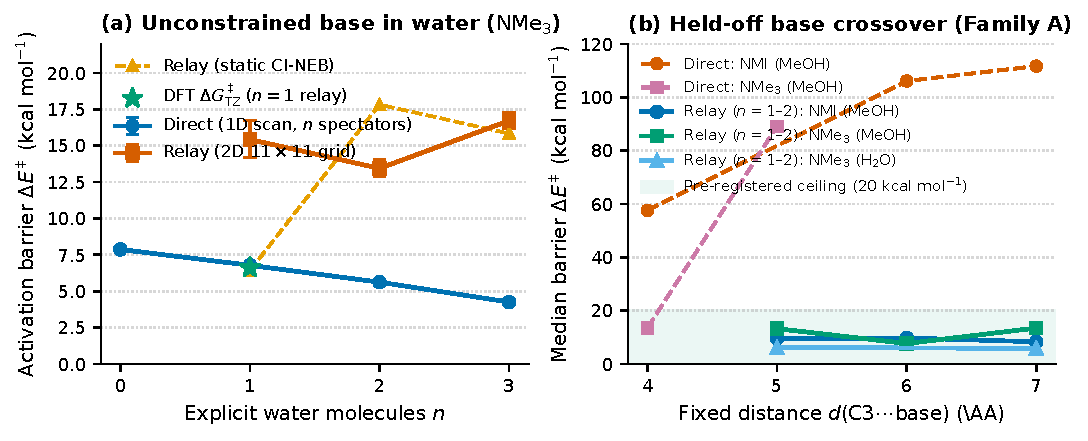
\includegraphics[width=\textwidth]{fig1_solution_vs_heldoff.pdf}
\caption{(a) Stage-1 solution-phase activation barriers ($\Delta E^\ddagger$, mean $\pm$ SD across $n_{\text{seed}} = 3$ seeds) for acetylacetone $\text{C3--H}$ deprotonation by $\text{NMe}_3$ in GFN2-xTB/ALPB(water) as a function of water wire length $n$, comparing 1D relaxed direct scans, 2D $11\times 11$ relay grids, static CI-NEB, and the $\omega$B97X-D3(BJ)/def2-TZVP//def2-SVP/IEF-PCM single-water relay transition state ($\Delta G^\ddagger_{\text{TZ}} = 6.61$\,kcal\,mol$^{-1}$). (b) Stage-1b Family~A distance crossover when the base ($\text{NMI}$ or $\text{NMe}_3$) is held at fixed distance $d(\text{C3}\cdots\text{base}) \in [4.0, 7.0]$\,\AA{}, showing the direct barrier spiking to $89.11$--$111.64$\,kcal\,mol$^{-1}$ at $d \ge 5.0$\,\AA{} while $1$--$2$-molecule water or methanol relays remain flat at $5.80$--$15.95$\,kcal\,mol$^{-1}$.}
\label{fig:fig1}
\end{figure}

As shown in Table~\ref{tab:stage1} and Figure~\ref{fig:fig1}a, when $\text{NMe}_3$ is free to move in solution, it compresses to $R_{\text{DA}}(\text{C3}\cdots\text{N}) = 2.70$\,\AA{} at the transition state, and the spectator waters solvate the developing enolate oxygens. Consequently, the direct-transfer barrier decreases monotonically with added spectator waters from $7.87 \pm 0.03$\,kcal\,mol$^{-1}$ ($n=0$) to $6.78 \pm 0.03$ ($n=1$), $5.62 \pm 0.06$ ($n=2$), and $4.25 \pm 0.16$\,kcal\,mol$^{-1}$ ($n=3$). By contrast, forcing the proton through the water wire in the relay topology yields barriers of $15.43 \pm 1.27$ ($n=1$), $13.44 \pm 0.58$ ($n=2$), and $16.72 \pm 0.57$\,kcal\,mol$^{-1}$ ($n=3$) on the $11\times 11$ 2D grid, with concerted transfer at $n=1$ and stepwise hydronium-like intermediates at $n=2, 3$. Only at $n=1$ do CI-NEB ($6.41 \pm 0.72$\,kcal\,mol$^{-1}$) and the $\omega$B97X-D3(BJ) DFT check ($\Delta E^\ddagger_{\text{SVP}} = 4.89$\,kcal\,mol$^{-1}$, $\Delta G^\ddagger_{\text{TZ}} = 6.61$\,kcal\,mol$^{-1}$, single imaginary mode $\nu^\ddagger = 210.0i$\,cm$^{-1}$) reach parity with direct transfer. Thus, Hypothesis~H1 is rejected for an unconstrained small base in bulk solution.

\subsection{Stage~1b: Bioinspired Levers That Rescue the Proton Relay}
Evaluating all 660 jobs of the Stage-1b screen (\texttt{data/stage1b\_screen\_summary.json}; 253 \texttt{ok}, 155 \texttt{geometry\_infeasible}, 110 \texttt{neb\_not\_converged}, 82 \texttt{product\_not\_minimum}, 35 \texttt{error}, 21 \texttt{timeout}, 4 \texttt{reactant\_not\_minimum}) confirmed that the 7-hydroxyquinoline positive control (Family~Q) passes in water ($n=2$: $20.79$\,kcal\,mol$^{-1}$; $n=3$: $12.54$\,kcal\,mol$^{-1}$; $n=0$ unviable) and revealed how each of the three bioinspired levers shifts the relay vs.\ direct balance (Table~\ref{tab:stage1b}, Figure~\ref{fig:fig1}b).

\begin{table}[htbp]
\centering
\caption{Selected Stage-1b bioinspired screening results (GFN2-xTB/ALPB median barriers across $\ge 2/3$ usable seeds, kcal\,mol$^{-1}$) across Family~A (held-off base at fixed distance $d$), Family~B (bifunctional shuttles on cyclohexa-2,4-dien-1-one $\to$ phenol), Family~C (\textit{all-cis} cyclohexane-1,3,5-triol wire), and Family~Q (7-hydroxyquinoline control).}
\label{tab:stage1b}
\footnotesize
\setlength{\tabcolsep}{4pt}
\resizebox{\textwidth}{!}{\begin{tabular}{@{}llcccccc@{}}
\toprule
Fam. & System / Condition & Solv. & $d$ (\AA{}) / Shuttle & Direct / Step & Relay $\Delta E^\ddagger$ ($n_{\text{best}}$) & $\Delta\Delta E^\ddagger$ (Relay$-$Ref) & Verdict \\
\midrule
A & $\text{acac} + \text{NMe}_3$ & MeOH & $d = 4.0$ & $13.43$ & --- & --- & No relay \\
A & $\text{acac} + \text{NMe}_3$ & MeOH & $d = 5.0$ & $89.11$ & $\mathbf{13.23}$ ($n=1$) & $\mathbf{-75.88}$ & \textbf{HIT} \\
A & $\text{acac} + \text{NMe}_3$ & $\text{H}_2\text{O}$ & $d = 5.0$ & \textit{unusable}$^{\text{a}}$ & $\mathbf{6.22}$ ($n=1$) & --- & Undetermined$^{\text{a}}$ \\
A & $\text{acac} + \text{NMe}_3$ & $\text{H}_2\text{O}$ & $d = 7.0$ & \textit{unusable}$^{\text{a}}$ & $\mathbf{5.80}$ ($n=2$) & --- & Undetermined$^{\text{a}}$ \\
A & $\text{acac} + \text{NMI}$ & $\text{H}_2\text{O}$ & $d = 5.0$ & $89.83$ & $\mathbf{15.95}$ ($n=1$) & $\mathbf{-73.88}$ & \textbf{HIT} \\
A & $\text{acac} + \text{NMI}$ & MeOH & $d = 6.0$ & $106.07$ & $\mathbf{9.74}$ ($n=1$) & $\mathbf{-96.33}$ & \textbf{HIT} \\
A & $\text{acac} + \text{NMI}$ & MeOH & $d = 7.0$ & $111.64$ & $\mathbf{8.30}$ ($n=2$) & $\mathbf{-103.34}$ & \textbf{HIT} \\
A & $\text{acac} + \text{AcO}^-$ & $\text{H}_2\text{O}$ & $d = 6.0$ & \textit{unusable}$^{\text{a}}$ & $\mathbf{12.00}$ ($n=1$) & --- & Undetermined$^{\text{a}}$ \\
\midrule
B & Dienone $\to$ phenol & $\text{H}_2\text{O}$ & None (intra) & --- & $46.73$ ($n=0$) & --- & Baseline \\
B & Dienone $\to$ phenol & $\text{H}_2\text{O}$ & $1\,\text{H}_2\text{O}$ & \textit{unusable} & $18.69$ ($n=1$) & $0.00$ (ref) & Baseline \\
B & Dienone $\to$ phenol & $\text{H}_2\text{O}$ & 2-Pyridone & $2.20$ (step) & $\mathbf{1.00}$ & $-1.20$ ($-17.69$ vs.\ $\text{H}_2\text{O}$) & Fast shuttle \\
B & Dienone $\to$ phenol & $\text{H}_2\text{O}$ & AcOH & $4.35$ (step) & $\mathbf{4.44}$ & $+0.10$ ($-14.25$ vs.\ $\text{H}_2\text{O}$) & Fast shuttle \\
\midrule
C & $\text{acac} + \text{NMe}_3 + \text{triol}$ & MeOH & \textit{cis}-1,3,5-Triol & $19.68$ (loose $w_3$) & $\mathbf{12.45}$ (3-hop) & $\mathbf{-7.23}$ vs.\ loose $w_3$ & Preorg.\ gain$^{\text{b}}$ \\
C & $\text{acac} + \text{AcO}^- + \text{triol}$ & MeOH & \textit{cis}-1,3,5-Triol & $18.86$ (loose $w_3$) & $\mathbf{10.52}$ (3-hop) & $\mathbf{-8.35}$ vs.\ loose $w_3$ & Preorg.\ gain$^{\text{b}}$ \\
\midrule
Q & 7-Hydroxyquinoline & $\text{H}_2\text{O}$ & $(\text{H}_2\text{O})_2$ / $(\text{H}_2\text{O})_3$ & \textit{unviable} ($n=0$) & $\mathbf{20.79}$ / $\mathbf{12.54}$ & Passes control & \textbf{PASS} \\
\bottomrule
\end{tabular}}
\begin{flushleft}
\footnotesize $^{\text{a}}$Direct transfer at $d \ge 5.0$\,\AA{} had $<2/3$ converged seeds (e.g., 1/3 converged at $108.32$\,kcal\,mol$^{-1}$ for $\text{AcO}^-$ at $d=6.0$\,\AA{} in water), so the pre-registered rule labels the pair \texttt{undetermined\_direct\_unusable} even though the relay converged across $\ge 2/3$ seeds at $5.80$--$18.06$\,kcal\,mol$^{-1}$. $^{\text{b}}$Marked \texttt{undetermined} under the joint rule because only $1/3$ direct-topology triol seeds converged ($7.92$ and $16.45$\,kcal\,mol$^{-1}$).
\end{flushleft}
\end{table}

\paragraph{Lever 1: Distance crossover when the base is held off the carbon acid (Family~A).}
At $d(\text{C3}\cdots\text{base}) = 4.0$\,\AA{}, direct transfer remains accessible ($9.17$--$57.56$\,kcal\,mol$^{-1}$) while an intercalated water molecule is sterically compressed. At $d = 5.0$\,\AA{}, a sharp crossover occurs: direct proton transfer without a bridge must cross a $>2.8$\,\AA{} gap, driving the direct barrier to $89.11$\,kcal\,mol$^{-1}$ ($\text{NMe}_3$, MeOH) and $89.83$\,kcal\,mol$^{-1}$ (NMI, water), whereas a single bridging water or methanol molecule ($n=1$) relays the proton with barriers of $13.23$ and $15.95$\,kcal\,mol$^{-1}$ (both formal \textbf{HITs}). At $d = 6.0$ and $7.0$\,\AA{}, the NMI direct barrier rises to $106.07$ and $111.64$\,kcal\,mol$^{-1}$, while $n=1$ and $n=2$ relays drop to $\mathbf{9.74}$ and $\mathbf{8.30}$\,kcal\,mol$^{-1}$ ($\Delta\Delta E^\ddagger = -96.33$ and $-103.34$\,kcal\,mol$^{-1}$). In water with $\text{NMe}_3$, the relay barrier remains flat at $6.22$\,kcal\,mol$^{-1}$ ($d=5.0$\,\AA{}, $n=1$) and $5.80$\,kcal\,mol$^{-1}$ ($d=7.0$\,\AA{}, $n=2$).

\paragraph{Lever 2 and Lever 3: Bifunctional shuttles (Family~B) and preorganised triol wire (Family~C).}
In the aromatising keto$\to$enol tautomerisation of cyclohexa-2,4-dien-1-one to phenol (Family~B), the unassisted intramolecular 1,3-proton shift has a barrier of $46.73$\,kcal\,mol$^{-1}$ in water, and a single water shuttle lowers it to $18.69$\,kcal\,mol$^{-1}$. Introducing 2-pyridone or acetic acid slashes the concerted cyclic relay barrier in water to $\mathbf{1.00}$ and $\mathbf{4.44}$\,kcal\,mol$^{-1}$ ($-17.69$ and $-14.25$\,kcal\,mol$^{-1}$ vs.\ water). Replacing three loose water molecules by the triaxial hydroxyl chain of \textit{all-cis} cyclohexane-1,3,5-triol (Family~C) lowers the 3-hop relay barrier in methanol from $19.68$ to $\mathbf{12.45}$\,kcal\,mol$^{-1}$ with $\text{NMe}_3$ ($\Delta\Delta E^\ddagger = -7.23$\,kcal\,mol$^{-1}$) and from $18.86$ to $\mathbf{10.52}$\,kcal\,mol$^{-1}$ with acetate ($\Delta\Delta E^\ddagger = -8.35$\,kcal\,mol$^{-1}$).

\subsection{Stage~1c: Non-Peptide Synthetic Systems---Bulky Bases and Metal Complexes}
To achieve the held-off relay regime in a non-peptide synthetic system \textbf{without any artificial distance restraints}, we evaluated 72 unconstrained 1D relaxed scans across bulky bases (DTBMP, TMP), amidine/guanidine organocatalysts (DBU, TBD), and tetrahedral Lewis-acid metal-diketone complexes ($[\text{MgCl}_2(\text{acac})]$ and $[\text{ZnCl}_2(\text{acac})]$) (\texttt{data/stage1c\_nonpeptide\_summary.json}, Table~\ref{tab:stage1c}, Figure~\ref{fig:fig3}).

\begin{table}[htbp]
\centering
\caption{Stage-1c unconstrained non-peptide proton-transfer barriers ($\Delta E^\ddagger$, kcal\,mol$^{-1}$, mean $\pm$ SD and median across $n_{\text{seed}} = 3$ seeds in GFN2-xTB/ALPB(water)), donor--acceptor distances $R_{\text{DA}}(\text{C3}\cdots\text{N})$ (\AA{}) in the relaxed reactant ($\text{R}$) and transition state ($\text{TS}$), and unconstrained product reaction energies ($\Delta E_{\text{rxn}}$, kcal\,mol$^{-1}$).}
\label{tab:stage1c}
\footnotesize
\setlength{\tabcolsep}{4pt}
\resizebox{\textwidth}{!}{\begin{tabular}{@{}llcccccc@{}}
\toprule
Fam. & Non-Peptide System & Topology ($n$) & $\Delta E^\ddagger$ Mean $\pm$ SD & Median $\Delta E^\ddagger$ & $R_{\text{DA}}(\text{R} \to \text{TS})$ (\AA{}) & Unconstrained $\Delta E_{\text{rxn}}$ & Outcome \\
\midrule
E1 & $\text{acac} + \text{DBU}$ (amidine) & Direct ($n=1$) & $3.10 \pm 1.31$ & $2.80$ & $2.99 \to 2.67$ & $-3.91$ & Direct contact wins \\
E1 & $\text{acac} + \text{DBU}$ (amidine) & Relay ($n=1$) & $9.37 \pm 0.39$ & $9.34$ & $5.52 \to 4.73$ & $-2.74$ & $+6.27$ vs.\ direct \\
E1 & $\text{acac} + \text{TMP}$ (piperidine) & Direct ($n=1$) & $7.00 \pm 2.40$ & $6.43$ & $3.10 \to 2.73$ & $+2.78$ & Direct contact wins \\
E1 & $\text{acac} + \text{TMP}$ (piperidine) & Relay ($n=1$) & $12.47 \pm 0.74$ & $12.69$ & $5.48 \to 4.74$ & $+0.69$ & $+5.47$ vs.\ direct \\
E1 & $\text{acac} + \text{DTBMP}$ ($2,6\text{-}t\text{Bu}_2\text{Py}$) & Direct ($n=0$) & $13.66 \pm 2.88$ & $12.00$ & $4.43 \to 2.72$ & $+1.88$ & Steric penalty $+6.9$ \\
E1 & $\text{acac} + \text{DTBMP}$ ($2,6\text{-}t\text{Bu}_2\text{Py}$) & Direct ($n=1$) & $12.22 \pm 0.75$ & $12.22$ & $4.51 \to 2.75$ & $+0.13$ & Forced compression \\
E1 & $\text{acac} + \text{DTBMP}$ ($2,6\text{-}t\text{Bu}_2\text{Py}$) & Relay ($n=1$) & $15.35 \pm 2.48$ & $15.90$ & $5.79 \to 5.03$ & $+1.82$ & Near-parity ($+3.13$) \\
E1 & $\text{acac} + \text{DTBMP}$ ($2,6\text{-}t\text{Bu}_2\text{Py}$) & Relay ($n=2$) & $13.51 \pm 0.24$ & $13.44$ & $7.72 \to 6.42$ & $-2.27$ & Beats $n=0$ mean \\
\midrule
E2 & $\text{acac} + \text{TBD}$ (guanidine) & Relay (cyclic) & $\mathbf{1.92 \pm 0.37}$ & $\mathbf{2.10}$ & $2.95 \to 2.71$ & $-4.95$ & Dual H-bond shuttle \\
E2 & $\text{acac} + \text{TBD}$ (guanidine) & Stepwise & $2.47 \pm 0.44$ & $2.28$ & $2.95 \to 2.65$ & $-5.44$ & $\Delta\Delta E^\ddagger = -0.55$ \\
\midrule
E3 & $[\text{MgCl}_2(\text{acac})] + \text{NMI}$ & Direct ($n=1$) & $0.49 \pm 0.28$ & $0.45$ & $2.78 \to 2.70$ & $-7.60$ & Small base contacts \\
E3 & $[\text{MgCl}_2(\text{acac})] + \text{NMI}$ & Relay ($n=1$) & $2.06 \pm 0.17$ & $2.09$ & $4.34 \to 4.31$ & $-17.39$ & Relay $\Delta E_{\text{rxn}}$ lower \\
E3 & $[\text{ZnCl}_2(\text{acac})] + \text{NMI}$ & Direct ($n=1$) & $1.95$ ($1/3$)$^{\text{a}}$ & $1.95$ & $2.96 \to 2.67$ & $-5.33$ & 2/3 R collapse \\
E3 & $[\text{ZnCl}_2(\text{acac})] + \text{NMI}$ & Relay ($n=1$) & $\mathbf{1.27 \pm 0.24}$ & $\mathbf{1.23}$ & $4.57 \to 4.45$ & $-24.13$ & \textbf{Relay wins} ($-0.68$) \\
E3 & $[\text{MgCl}_2(\text{acac})] + \text{DTBMP}$ & Direct ($n=1$) & $10.93 \pm 5.11$ & $10.58$ & $4.45 \to 3.08$ & $-12.06$ & Steric clash with $\text{MgCl}_2$ \\
E3 & $[\text{MgCl}_2(\text{acac})] + \text{DTBMP}$ & Relay ($n=1$) & $\mathbf{5.87 \pm 3.33}$ & $\mathbf{4.39}$ & $5.58 \to 5.01$ & $-19.82$ & \textbf{Relay wins} ($\mathbf{-6.19}$ med) \\
E3 & $[\text{ZnCl}_2(\text{acac})] + \text{DTBMP}$ & Direct ($n=1$) & $5.70 \pm 2.52$ & $6.29$ & $4.51 \to 3.16$ & $-18.88$ & Steric clash with $\text{ZnCl}_2$ \\
E3 & $[\text{ZnCl}_2(\text{acac})] + \text{DTBMP}$ & Relay ($n=1$) & $\mathbf{3.06 \pm 2.18}$ & $\mathbf{1.82}$ & $5.74 \to 4.91$ & $-20.59$ & \textbf{Relay wins} ($\mathbf{-4.47}$ med) \\
\bottomrule
\end{tabular}}
\begin{flushleft}
\footnotesize $^{\text{a}}$For $[\text{ZnCl}_2(\text{acac})] + \text{NMI}$ direct, 2/3 seeds transferred the proton barrierlessly during reactant relaxation (\texttt{reactant\_not\_minimum}).
\end{flushleft}
\end{table}

\begin{figure}[htbp]
\centering
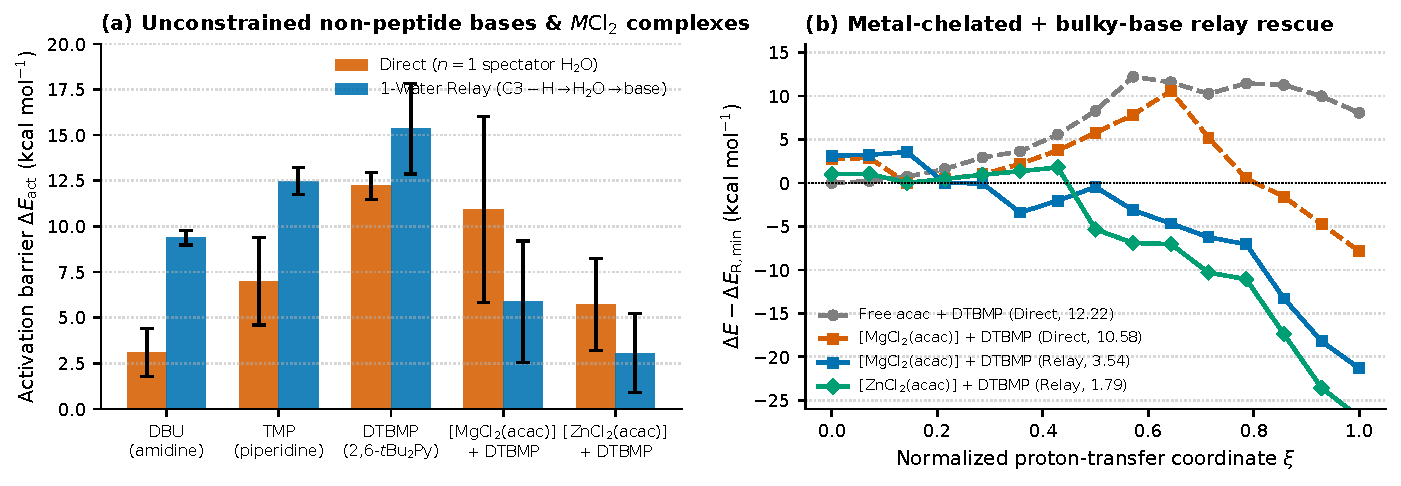
\includegraphics[width=\textwidth]{fig3_nonpeptide_complexes.pdf}
\caption{(a) Stage-1c unconstrained activation barriers ($\Delta E^\ddagger$, mean $\pm$ SD across $n_{\text{seed}} = 3$ seeds in GFN2-xTB/ALPB(water)) comparing composition-matched direct ($n=1$ spectator water) and 1-water relay pathways across unencumbered amidine DBU, hindered piperidine TMP, bulky pyridine DTBMP, and Lewis-acid metal-chelated complexes $[\text{MgCl}_2(\text{acac})] + \text{DTBMP}$ and $[\text{ZnCl}_2(\text{acac})] + \text{DTBMP}$. (b) Relaxed 15-point 1D proton-transfer energy profiles showing how combining $M\text{Cl}_2$ chelation with bulky DTBMP lowers the 1-water relay barrier from $12.22$--$15.35$\,kcal\,mol$^{-1}$ (free acac) to $3.54$\,kcal\,mol$^{-1}$ ($\text{MgCl}_2$, seed $s_2$) and $1.79$\,kcal\,mol$^{-1}$ ($\text{ZnCl}_2$, seed $s_2$), beating direct transfer without artificial distance constraints.}
\label{fig:fig3}
\end{figure}

Three design principles emerge from the Stage-1c non-peptide systems (Table~\ref{tab:stage1c}, Figure~\ref{fig:fig3}):
\begin{enumerate}
\item \textbf{Steric bulk on the base alone increases the direct barrier to near-parity with a 2-water relay:}
Whereas unhindered bicyclic DBU approaches acetylacetone to $R_{\text{DA}}(\text{R}) = 2.99$\,\AA{} and transfers the proton directly at $3.10 \pm 1.31$\,kcal\,mol$^{-1}$ (vs.\ $9.37 \pm 0.39$\,kcal\,mol$^{-1}$ for the 1-water relay), the flanking \textit{tert}-butyl groups of DTBMP hold the pyridine ring at $R_{\text{DA}}(\text{R}) = 4.43$--$4.51$\,\AA{} in the relaxed reactant. Forcing DTBMP into direct contact ($R_{\text{DA}}(\text{TS}) = 2.72$--$2.75$\,\AA{}) costs $12.22 \pm 0.75$ ($n=1$) to $13.66 \pm 2.88$\,kcal\,mol$^{-1}$ ($n=0$), virtually indistinguishable from the unconstrained 2-water relay ($13.51 \pm 0.24$\,kcal\,mol$^{-1}$ at $R_{\text{DA}}(\text{TS}) = 6.42$\,\AA{}, where the two water molecules slip between the \textit{tert}-butyl groups and stabilise the product by $\Delta E_{\text{rxn}} = -2.27$ vs.\ $+1.88$\,kcal\,mol$^{-1}$).
\item \textbf{Bicyclic guanidine TBD acts as a sub-$2$\,kcal\,mol$^{-1}$ bifunctional shuttle on $\beta$-diketones:}
On acetylacetone, the bicyclic guanidine TBD forms a dual hydrogen-bonded complex ($R_{\text{DA}} = 2.95$\,\AA{}) that executes concerted keto$\to$enol relay tautomerisation with a barrier of $\mathbf{1.92 \pm 0.37}$\,kcal\,mol$^{-1}$ (vs.\ $2.47 \pm 0.44$\,kcal\,mol$^{-1}$ stepwise, and $25.14$\,kcal\,mol$^{-1}$ for a single water molecule in Stage~1b).
\item \textbf{Synergy of Lewis-acid metal chelation ($[\text{MgCl}_2(\text{acac})]$, $[\text{ZnCl}_2(\text{acac})]$) and a bulky base (DTBMP) flips the preference to the water relay without artificial constraints:}
Chelating acetylacetone to $\text{MgCl}_2$ or $\text{ZnCl}_2$ both acidifies the $\text{C3--H}$ bond and increases steric congestion around the $\beta$-diketone core. When paired with a small base (NMI), NMI can still approach $\text{MgCl}_2$-chelated $\text{C3--H}$ to $R_{\text{DA}}(\text{TS}) = 2.70$\,\AA{} ($0.49 \pm 0.28$\,kcal\,mol$^{-1}$ direct vs.\ $2.06 \pm 0.17$\,kcal\,mol$^{-1}$ relay). However, when $[\text{MgCl}_2(\text{acac})]$ or $[\text{ZnCl}_2(\text{acac})]$ is paired with bulky DTBMP, steric repulsion between the $M\text{Cl}_2(\text{acac})$ complex and the 2,6-di-\textit{tert}-butyl groups prevents close N--C3 contact ($R_{\text{DA}}(\text{TS}) = 3.08$--$3.16$\,\AA{} in the direct path), imposing a direct barrier of $10.93 \pm 5.11$\,kcal\,mol$^{-1}$ (median $10.58$) for $\text{MgCl}_2$ and $5.70 \pm 2.52$\,kcal\,mol$^{-1}$ (median $6.29$) for $\text{ZnCl}_2$. Inserting a single bridging water molecule allows DTBMP to remain at its unstrained distance of $R_{\text{DA}}(\text{TS}) = 4.91$--$5.01$\,\AA{}, dropping the 1-water relay barrier to $\mathbf{5.87 \pm 3.33}$\,kcal\,mol$^{-1}$ (median $\mathbf{4.39}$\,kcal\,mol$^{-1}$, $\Delta\Delta E^\ddagger_{\text{med}} = -6.19$\,kcal\,mol$^{-1}$, $\Delta E_{\text{rxn}} = -19.82$\,kcal\,mol$^{-1}$) for $[\text{MgCl}_2(\text{acac})]$ and to $\mathbf{3.06 \pm 2.18}$\,kcal\,mol$^{-1}$ (median $\mathbf{1.82}$\,kcal\,mol$^{-1}$, $\Delta\Delta E^\ddagger_{\text{med}} = -4.47$\,kcal\,mol$^{-1}$, $\Delta E_{\text{rxn}} = -20.59$\,kcal\,mol$^{-1}$) for $[\text{ZnCl}_2(\text{acac})]$.
\end{enumerate}

\subsection{Stage~2: Proton Hopping in the TcmN ARO/CYC Enzyme Pocket (\texttt{3TVQ})}
To test whether an authentic polyketide cyclase active site realises these same geometric and electrostatic principles, we analysed the 241-atom QM cluster of TcmN ARO/CYC bound to \texttt{DQH} (PDB \texttt{3TVQ}, $1.67$\,\AA{} resolution). Constrained reactant relaxation with ASE \texttt{FixAtoms} on the 24 terminal $\text{C}_\alpha$ and H-cap atoms converged in 145 BFGS steps (\texttt{58.2}\,s wall, \texttt{fmax = 0.0479}\,eV\,\AA$^{-1}$) with \textbf{zero boundary drift} ($0.000000$\,\AA{} on all 24 fixed atoms; all-atom RMSD $= 0.445$\,\AA{} from crystal coordinates) and a clean HOMO--LUMO gap of $0.828$\,eV in ALPB(water).

\begin{table}[htbp]
\centering
\caption{Relaxed 1D proton-transfer scan barriers ($\Delta E^\ddagger$, kcal\,mol$^{-1}$) and unconstrained product reaction energies ($\Delta E_{\text{rxn}}$, kcal\,mol$^{-1}$) in the 241--244-atom TcmN ARO/CYC enzyme-pocket QM cluster (PDB \texttt{3TVQ}, GFN2-xTB/ALPB(water), 24 $\text{C}_\alpha$/cap atoms frozen) across three independent H-bond orientation seeds ($s_7, s_{11}, s_{13}$) and two $\text{His124}$ protonation states (neutral $\text{HIE}^0$ vs.\ cationic $\text{HIP}^+$).}
\label{tab:pocket}
\footnotesize
\setlength{\tabcolsep}{4.5pt}
\resizebox{\textwidth}{!}{\begin{tabular}{@{}llcccccc@{}}
\toprule
Channel & Pocket Pathway & $s_7$ & $s_{11}$ & $s_{13}$ & \textbf{3-Seed Mean $\pm$ SD} & $\text{His124}^+$ (\texttt{HIP}) & Unconstrained $\Delta E_{\text{rxn}}$ ($s_7$) \\
\midrule
Direct C10 & $\text{DQH:C10--H24} \to \text{Asp57:OD2}$ & $35.98$ & $34.36$ & $36.46$ & $\mathbf{35.60 \pm 1.10}$ & $33.66$ & $+20.39$ (stable min) \\
C10 Relay & $\text{DQH:C10--H24} \to \text{W999} \to \text{Asp57:OD2}$ & $27.96$ & --- & --- & $\mathbf{27.96}$ (1 seed) & --- & $+13.58$ (stable min) \\
2-Water Wire & $\text{DQH:O27--H31} \to \text{W259} \to \text{W266} \to \text{His128}$ & $14.56$ & $11.33$ & $11.29$ & $\mathbf{12.39 \pm 1.88}$ & $\mathbf{7.08}$ & $-2.64$ (stable min) \\
1-Water Wire & $\text{DQH:O27--H31} \to \text{W266} \to \text{His128:NE2}$ & $7.01$ & $14.60$ & $8.49$ & $\mathbf{10.03 \pm 4.02}$ & $\mathbf{6.74}$ & $-0.48$ (stable min)$^{\text{a}}$ \\
\bottomrule
\end{tabular}}
\begin{flushleft}
\footnotesize $^{\text{a}}$With cationic $\text{His124}^+$ (\texttt{HIP}, total cluster charge $+1$), the 1-water relay reaction energy is $\Delta E_{\text{rxn}} = -4.46$\,kcal\,mol$^{-1}$ and the 3-seed neutral median is $8.49$\,kcal\,mol$^{-1}$.
\end{flushleft}
\end{table}

\begin{figure}[htbp]
\centering
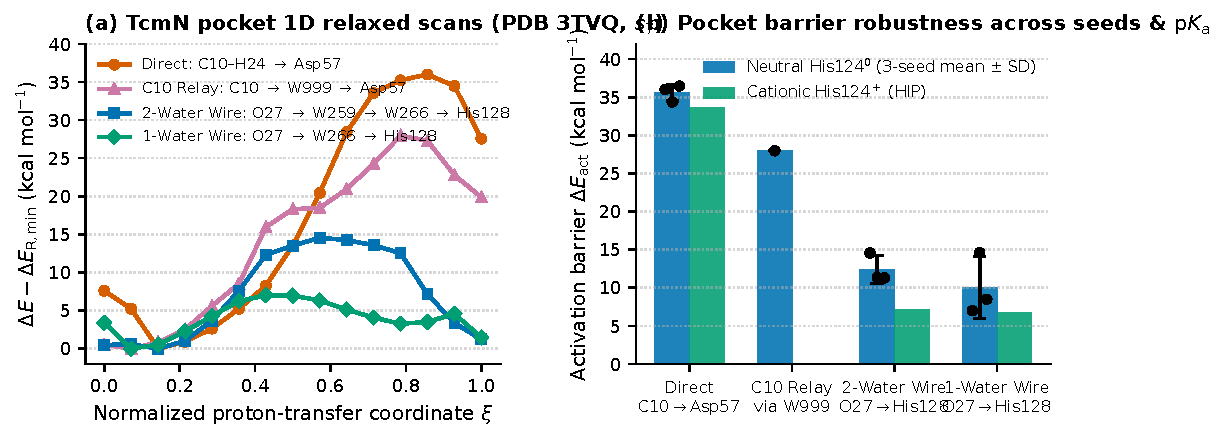
\includegraphics[width=\textwidth]{fig2_tcmn_pocket_profiles.pdf}
\caption{(a) Relaxed 15-point 1D proton-transfer energy profiles ($\Delta E - \Delta E_{\text{R,min}}$, GFN2-xTB/ALPB(water), seed $s_7$) in the 241--244-atom TcmN ARO/CYC active-site QM cluster (PDB \texttt{3TVQ}) across the four studied pathways. (b) Barrier comparison across three independent hydrogen-bond orientation seeds ($s_7, s_{11}, s_{13}$, mean $\pm$ SD with individual seed points overlaid) and the cationic $\text{His124}^+$ (\texttt{HIP}) protonation state.}
\label{fig:fig2}
\end{figure}

Inspection of the relaxed \texttt{3TVQ} active-site geometry and the 15-point 1D scans (Table~\ref{tab:pocket}, Figure~\ref{fig:fig2}) reveals three central mechanistic results:
\begin{enumerate}
\item \textbf{Geometric blocking of direct carbon-acid deprotonation ($\Delta E^\ddagger = 35.60 \pm 1.10$\,kcal\,mol$^{-1}$):}
Although the carboxylate oxygen $\text{Asp57:OD2}$ sits $3.325$\,\AA{} from the carbon acid $\text{DQH:C10}$ ($\alpha$ to the $\text{C9=O13}$ carbonyl), the pocket holds the $\text{C10--H24}$ bond at an acute angle to $\text{Asp57:OD2}$ ($\angle\text{H24--C10--OD2} = 55.9^\circ$, $d(\text{H24}\cdots\text{OD2}) = 2.856$\,\AA{}), while $\text{Asp57}$ is rigidly locked by hydrogen bonds from $\text{Trp63:HE1}$ ($1.820$\,\AA{}) and the $\text{Asn59:H}$ backbone amide ($1.738$\,\AA{} to $\text{OD1}$). Forcing direct $\text{C10--H24}\to\text{Asp57:OD2}$ transfer therefore requires $35.60 \pm 1.10$\,kcal\,mol$^{-1}$ across the three neutral seeds ($33.66$\,kcal\,mol$^{-1}$ with $\text{His124}^+$), leading to a high-energy enolate minimum at $\Delta E_{\text{rxn}} = +20.39$\,kcal\,mol$^{-1}$ ($d(\text{OD2--H24}) = 1.009$\,\AA{}, $\text{C10=C9}$ shortened from $1.521$ to $1.350$\,\AA{}).
\item \textbf{Rescue of carbon-acid deprotonation by a single cavity water ($\Delta\Delta E^\ddagger = -8.02$\,kcal\,mol$^{-1}$):}
Cavity analysis around $\text{C10--H24}$ identifies an unoccluded pocket site at $d(\text{H24}\cdots\text{O}) = 1.89$\,\AA{} and $d(\text{O}\cdots\text{Asp57:OD2}) = 2.67$\,\AA{} ($>2.45$\,\AA{} clearance from all surrounding heavy atoms). Inserting a single bridging water ($\text{HOH999}$, 244-atom cluster) and scanning the tethered 2-hop relay ($\text{DQH:C10--H24} \to \text{HOH999} \to \text{Asp57:OD2}$) lowers the forward barrier by $8.02$\,kcal\,mol$^{-1}$ to $\mathbf{27.96}$\,kcal\,mol$^{-1}$ and stabilises the unconstrained enolate product minimum by $6.81$\,kcal\,mol$^{-1}$ ($\Delta E_{\text{rxn}} = +13.58$\,kcal\,mol$^{-1}$).
\item \textbf{Low-barrier, reversible proton conduction along the crystallographic water wire ($\Delta E^\ddagger = 6.74$--$14.56$\,kcal\,mol$^{-1}$):}
In \texttt{3TVQ}, the catalytic base $\text{His128:NE2}$ is held $4.024$\,\AA{} from the substrate $\text{O27}$ oxygen and $3.893$\,\AA{} from $\text{C10}$---precisely the held-off distance regime ($d \ge 4$--$5$\,\AA{}) identified in Stage-1b Family~A and Stage-1c Family~E3. The crystallographic water wire bridges this gap through $\text{HOH259}$ and $\text{HOH266}$. Along the 2-water wire ($\text{DQH:O27--H31}\to\text{W259}\to\text{W266}\to\text{His128}$), the 3-hop Grotthuss relay proceeds with a barrier of $\mathbf{12.39 \pm 1.88}$\,kcal\,mol$^{-1}$ (median $11.33$\,kcal\,mol$^{-1}$; paired difference vs.\ direct $\text{C10}\to\text{Asp57}$ across the three seeds $\Delta\Delta E^\ddagger = -23.21 \pm 1.84$\,kcal\,mol$^{-1}$) to a stable zwitterionic product minimum ($\text{DQH:O27}^-\cdots\text{HOH266}\cdots\text{His128H}^+$, $\Delta E_{\text{rxn}} = -2.64$\,kcal\,mol$^{-1}$). Along the 1-water crystallographic shortcut ($\text{DQH:O27--H31}\to\text{W266}\to\text{His128}$, enabled by $d(\text{O27}\cdots\text{HOH266:O}) = 2.745$\,\AA{} and $d(\text{HOH266:O}\cdots\text{His128:NE2}) = 2.756$\,\AA{}), the concerted 2-hop relay barrier drops to a median of $\mathbf{8.49}$\,kcal\,mol$^{-1}$ ($7.01$\,kcal\,mol$^{-1}$ in $s_7$, $\Delta E_{\text{rxn}} = -0.48$\,kcal\,mol$^{-1}$; paired difference vs.\ direct $\Delta\Delta E^\ddagger = -25.57 \pm 4.92$\,kcal\,mol$^{-1}$), where the developing $\text{O27}^-$ oxyanion is chelatively stabilised by $\text{HOH259}$ ($1.621$\,\AA{}) and $\text{HOH234}$ ($1.678$\,\AA{}). Protonating the adjacent $\text{His124}$ residue ($\text{HIP}^+$ variant) provides additional electrostatic oxyanion stabilisation, lowering the 2-water and 1-water relay barriers to $\mathbf{7.08}$ and $\mathbf{6.74}$\,kcal\,mol$^{-1}$ ($\Delta E_{\text{rxn}} = -4.46$\,kcal\,mol$^{-1}$).
\end{enumerate}

\section{Scope Constraints and Testable Predictions}
The majority of the 1{,}142 reaction-path calculations reported here are semi-empirical GFN2-xTB/ALPB electronic energies without zero-point vibrational energy or conformational entropy corrections, complemented by one full $\omega$B97X-D3(BJ)/def2-TZVP//def2-SVP/IEF-PCM transition state ($\Delta G^\ddagger = 6.61$\,kcal\,mol$^{-1}$ for the $n=1$ $\text{NMe}_3$/water relay). Furthermore, the \texttt{3TVQ} crystal structure captures TcmN bound to the flavanonol product mimic \texttt{DQH} rather than the reactive linear decaketide intermediate, so the $\text{C10--H24}$ bond is less acidic than an open-chain poly-$\beta$-carbonyl methylene flanked by two ketones. Nevertheless, the convergence of the Stage-1b/1c synthetic screens and the \texttt{3TVQ} enzyme-pocket scans yields three falsifiable predictions for continuous-flow and enzymatic experiments:
\begin{enumerate}
\item \textbf{Non-peptide soft-enolisation relay catalysis ($M\text{Cl}_2 + \text{DTBMP} + \text{H}_2\text{O}$):} Whereas unhindered amines ($\text{NMe}_3$, DBU, NMI) deprotonate $\beta$-dicarbonyls by direct contact ($R_{\text{DA}} \approx 2.7$\,\AA{}), combining a chelating Lewis acid ($\text{MgCl}_2$ or $\text{ZnCl}_2$) with a sterically encumbered pyridine base ($2,6$-di-\textit{tert}-butyl-4-methylpyridine, DTBMP) and $1$--$2$ equivalents of water in flow is predicted to switch the mechanism to a low-barrier water-bridged relay ($\Delta E^\ddagger_{\text{med}} = 1.82$--$4.39$\,kcal\,mol$^{-1}$ vs.\ $6.29$--$10.58$\,kcal\,mol$^{-1}$ direct).
\item \textbf{Bifunctional shuttle catalysis in flow:} Adding $10$--$20$\,mol\% of a bifunctional tautomeric catalyst (2-pyridone, acetic acid, or bicyclic guanidine TBD, $\Delta E^\ddagger = 1.00$--$4.44$\,kcal\,mol$^{-1}$) to base-induced polyketide cyclisations is predicted to accelerate keto--enol tautomerisation and post-aldol aromatisation by $>14$\,kcal\,mol$^{-1}$ in activation barrier over water alone.
\item \textbf{Proton-inventory and mutagenesis signatures in TcmN:} Mutating $\text{His128}$ to Phe/Ala or disrupting the $\text{HOH259/HOH266}$ water wire in TcmN is predicted to abolish rapid $\text{O27}$ proton shuttling, while $\text{D}_2\text{O}$ proton-inventory measurements \cite{venkatasubban1984} on the wild-type enzyme should exhibit quadratic/cubic curvature characteristic of a 2-to-3-proton Grotthuss relay.
\end{enumerate}

\section{Conclusion}
By testing the polyketide proton-relay hypothesis across unconstrained solution complexes (Stage~1), pre-registered bioinspired model systems (Stage~1b), non-peptide bulky-base and metal-chelated complexes (Stage~1c), and a 241--244-atom QM cluster of the TcmN ARO/CYC active site (Stage~2, PDB \texttt{3TVQ}), we resolve when Grotthuss proton hopping operates in polyketide cyclisations. A freely diffusing small base in solution does not use a multi-water wire because direct donor--acceptor contact ($R_{\text{DA}} \approx 2.7$\,\AA{}) is barrier-minimal ($3.10$--$6.78$\,kcal\,mol$^{-1}$). Conversely, holding the base $\ge 4.9$--$5.0$\,\AA{} from the donor---either through holonomic tethering, non-peptide Lewis-acid chelation paired with a 2,6-di-\textit{tert}-butylpyridine base ($[\text{MgCl}_2(\text{acac})]/[\text{ZnCl}_2(\text{acac})] + \text{DTBMP}$), or an enzymatic active site---or supplying a preorganised/bifunctional hydrogen-bond chain (2-pyridone, TBD, \textit{all-cis} cyclohexane-1,3,5-triol, or the crystallographic $\text{HOH259--HOH266--His128}$ wire of TcmN) rescues the proton relay, achieving $1.82$--$5.87$\,kcal\,mol$^{-1}$ barriers in synthetic metal complexes and $6.74$--$14.56$\,kcal\,mol$^{-1}$ proton conduction in the enzyme pocket.

\section*{Data and Code Availability}
All source code, RDKit/PubChem structure validators, cluster builders, GFN2-xTB/ALPB and PySCF/geomeTRIC runners, 3D coordinates (\texttt{cluster\_3TVQ.xyz}), and JSON summary datasets (\texttt{stage1\_summary.json}, \texttt{stage1b\_screen\_summary.json}, \texttt{stage1c\_nonpeptide\_summary.json}, \texttt{pocket\_3TVQ\_scans\_summary.json}) are openly available under the MIT licence at \url{https://github.com/sailblack-research/proton-hopping-mechanism-sim}.

\section*{Conflicts of Interest}
The author declares no competing financial interests.

\raggedright
\begin{thebibliography}{99}
\bibitem{myers2005sci} M.\,G.\ Charest, C.\,D.\ Lerner, J.\,D.\ Brubaker, D.\,R.\ Siegel, A.\,G.\ Myers, \textit{Science} \textbf{2005}, \textit{308}, 395--398, \href{https://doi.org/10.1126/science.1109755}{doi:10.1126/science.1109755}.
\bibitem{myers2005jacs} M.\,G.\ Charest, D.\,R.\ Siegel, A.\,G.\ Myers, \textit{J.\ Am.\ Chem.\ Soc.} \textbf{2005}, \textit{127}, 8292--8293, \href{https://doi.org/10.1021/ja052151d}{doi:10.1021/ja052151d}.
\bibitem{myers2001} A.\,G.\ Myers, D.\,R.\ Siegel, D.\,J.\ Buzard, M.\,G.\ Charest, \textit{Org.\ Lett.} \textbf{2001}, \textit{3}, 2923--2926, \href{https://doi.org/10.1021/ol010142o}{doi:10.1021/ol010142o}.
\bibitem{shen1995} B.\ Shen, R.\,G.\ Summers, H.\ Wendt, C.\,R.\ Hutchinson, \textit{J.\ Am.\ Chem.\ Soc.} \textbf{1995}, \textit{117}, 6811--6821, \href{https://doi.org/10.1021/ja00131a002}{doi:10.1021/ja00131a002}.
\bibitem{shen1996} B.\ Shen, C.\,R.\ Hutchinson, \textit{Proc.\ Natl.\ Acad.\ Sci.\ USA} \textbf{1996}, \textit{93}, 6600--6604, \href{https://doi.org/10.1073/pnas.93.13.6600}{doi:10.1073/pnas.93.13.6600}.
\bibitem{ames2008} B.\,D.\ Ames, K.\ Korman, W.\ Zhang, C.\,D.\ Smith, Y.\ Tang, S.-C.\ Tsai, \textit{Proc.\ Natl.\ Acad.\ Sci.\ USA} \textbf{2008}, \textit{105}, 5349--5354, \href{https://doi.org/10.1073/pnas.0709223105}{doi:10.1073/pnas.0709223105}.
\bibitem{zhou2010} H.\ Zhou, Y.\ Li, Y.\ Tang, \textit{Nat.\ Prod.\ Rep.} \textbf{2010}, \textit{27}, 839--868, \href{https://doi.org/10.1039/b911518h}{doi:10.1039/b911518h}.
\bibitem{ames2011} B.\,D.\ Ames, C.\ Nguyen, J.\ Bruegger, P.\ Smith, W.\ Xu, S.\ Ma, E.\ Wong, S.\,H.\ Wong, X.\ Xie, J.\,W.\ Li, J.\,C.\ Vederas, Y.\ Tang, S.-C.\ Tsai, \textit{Biochemistry} \textbf{2011}, \textit{50}, 8392--8406, \href{https://doi.org/10.1021/bi200593m}{doi:10.1021/bi200593m}.
\bibitem{lee2012} M.-Y.\ Lee, B.\,D.\ Ames, S.-C.\ Tsai, \textit{Biochemistry} \textbf{2012}, \textit{51}, 3079--3091, \href{https://doi.org/10.1021/bi201705q}{doi:10.1021/bi201705q}.
\bibitem{caldara2015} G.\ Caldara-Festin, D.\,R.\ Jackson, J.\,F.\ Barajas, T.\,P.\ Valentic, A.\,B.\ Patel, S.\ Aguilar, M.\ Nguyen, M.\ Vo, A.\ Khanna, E.\ Sasaki, H.-w.\ Liu, S.-C.\ Tsai, \textit{Proc.\ Natl.\ Acad.\ Sci.\ USA} \textbf{2015}, \textit{112}, E6844--E6851, \href{https://doi.org/10.1073/pnas.1512976112}{doi:10.1073/pnas.1512976112}.
\bibitem{harris1975} T.\,M.\ Harris, P.\,J.\ Wittek, \textit{J.\ Am.\ Chem.\ Soc.} \textbf{1975}, \textit{97}, 3270--3271, \href{https://doi.org/10.1021/ja00844a085}{doi:10.1021/ja00844a085}.
\bibitem{hayat1999} N.\ Hayat, \textit{Synthese von Anthrachinon-Antibiotika durch biomimetische Cyclisierung von Polyketiden}, Dissertation, Universit\"at-GH Paderborn, \textbf{1999}, URN \texttt{urn:nbn:de:hbz:466-1999010146}.
\bibitem{krohn1999} K.\ Krohn, S.\ Bernhard, \textit{Eur.\ J.\ Org.\ Chem.} \textbf{1999}, 3099--3103, \href{https://doi.org/10.1002/(SICI)1099-0690(199911)1999:11<3099::AID-EJOC3099>3.0.CO;2-2}{doi:10.1002/(SICI)1099-0690(199911)1999:11<3099::AID-EJOC3099>3.0.CO;2-2}.
\bibitem{krohn2000} K.\ Krohn, S.\ Bernhard, U.\ Fl\"orke, N.\ Hayat, \textit{J.\ Org.\ Chem.} \textbf{2000}, \textit{65}, 3218--3222, \href{https://doi.org/10.1021/jo9918089}{doi:10.1021/jo9918089}.
\bibitem{krohn2002} K.\ Krohn, \textit{Eur.\ J.\ Org.\ Chem.} \textbf{2002}, 1351--1362, \href{https://doi.org/10.1002/1099-0690(200204)2002:8<1351::AID-EJOC1351>3.0.CO;2-D}{doi:10.1002/1099-0690(200204)2002:8<1351::AID-EJOC1351>3.0.CO;2-D}.
\bibitem{barrett2018} T.\,K.\ Ma, D.\,C.\ Elliott, S.\ Reid, A.\,J.\,P.\ White, P.\,J.\ Parsons, A.\,G.\,M.\ Barrett, \textit{J.\ Org.\ Chem.} \textbf{2018}, \textit{83}, 13276--13286, \href{https://doi.org/10.1021/acs.joc.8b02095}{doi:10.1021/acs.joc.8b02095}.
\bibitem{barrett2019} T.\,K.\ Ma, P.\,J.\ Parsons, A.\,G.\,M.\ Barrett, \textit{J.\ Org.\ Chem.} \textbf{2019}, \textit{84}, 4961--4970, \href{https://doi.org/10.1021/acs.joc.9b00142}{doi:10.1021/acs.joc.9b00142}.
\bibitem{sparr2020} V.\,C.\ F\"aseke, F.\,C.\ Raps, C.\ Sparr, \textit{Angew.\ Chem.\ Int.\ Ed.} \textbf{2020}, \textit{59}, 6975--6983, \href{https://doi.org/10.1002/anie.201915055}{doi:10.1002/anie.201915055}.
\bibitem{kleber2020} J.\,M.\ Kleber, \textit{F5-2 API Synthesis Plan}, \textbf{2020}, \href{https://doi.org/10.13140/RG.2.2.23579.28965}{doi:10.13140/RG.2.2.23579.28965}.
\bibitem{agmon1995} N.\ Agmon, \textit{Chem.\ Phys.\ Lett.} \textbf{1995}, \textit{244}, 456--462, \href{https://doi.org/10.1016/0009-2614(95)00905-J}{doi:10.1016/0009-2614(95)00905-J}.
\bibitem{marx1999} D.\ Marx, M.\,E.\ Tuckerman, J.\ Hutter, M.\ Parrinello, \textit{Nature} \textbf{1999}, \textit{397}, 601--604, \href{https://doi.org/10.1038/17579}{doi:10.1038/17579}.
\bibitem{cukierman2006} S.\ Cukierman, \textit{Biochim.\ Biophys.\ Acta Bioenerg.} \textbf{2006}, \textit{1757}, 876--885, \href{https://doi.org/10.1016/j.bbabio.2005.12.001}{doi:10.1016/j.bbabio.2005.12.001}.
\bibitem{sultana2004} A.\ Sultana, P.\ Kallio, A.\ Jansson, J.-S.\ Wang, J.\ Niemi, P.\ M\"ants\"al\"a, G.\ Schneider, \textit{EMBO J.} \textbf{2004}, \textit{23}, 1911--1921, \href{https://doi.org/10.1038/sj.emboj.7600201}{doi:10.1038/sj.emboj.7600201}.
\bibitem{silverman1988} D.\,N.\ Silverman, S.\ Lindskog, \textit{Acc.\ Chem.\ Res.} \textbf{1988}, \textit{21}, 30--36, \href{https://doi.org/10.1021/ar00145a005}{doi:10.1021/ar00145a005}.
\bibitem{riccardi2006} D.\ Riccardi, P.\ K\"onig, X.\ Prat-Resina, H.\ Yu, M.\ Elstner, T.\ Frauenheim, Q.\ Cui, \textit{J.\ Am.\ Chem.\ Soc.} \textbf{2006}, \textit{128}, 16302--16311, \href{https://doi.org/10.1021/ja065451j}{doi:10.1021/ja065451j}.
\bibitem{kirby1980} A.\,J.\ Kirby, \textit{Adv.\ Phys.\ Org.\ Chem.} \textbf{1980}, \textit{17}, 183--278, \href{https://doi.org/10.1016/S0065-3160(08)60129-X}{doi:10.1016/S0065-3160(08)60129-X}.
\bibitem{odella2018} E.\ Odella, S.\,J.\ Mora, B.\,L.\ Wadsworth, M.\,T.\ Huynh, J.\,J.\ Goings, P.\,A.\ Liddell, T.\,L.\ Groy, M.\ Gervaldo, L.\,E.\ Sereno, D.\ Gust, T.\,A.\ Moore, G.\,F.\ Moore, S.\ Hammes-Schiffer, A.\,L.\ Moore, \textit{J.\ Am.\ Chem.\ Soc.} \textbf{2018}, \textit{140}, 15450--15460, \href{https://doi.org/10.1021/jacs.8b09724}{doi:10.1021/jacs.8b09724}.
\bibitem{hammes2015} S.\ Hammes-Schiffer, \textit{J.\ Am.\ Chem.\ Soc.} \textbf{2015}, \textit{137}, 8860--8871, \href{https://doi.org/10.1021/jacs.5b04087}{doi:10.1021/jacs.5b04087}.
\bibitem{alagona2010} G.\ Alagona, C.\ Ghio, P.\,I.\ Nagy, \textit{Phys.\ Chem.\ Chem.\ Phys.} \textbf{2010}, \textit{12}, 10173--10188, \href{https://doi.org/10.1039/c003999c}{doi:10.1039/c003999c}.
\bibitem{zotova2007} N.\ Zotova, A.\ Franzke, A.\ Armstrong, D.\,G.\ Blackmond, \textit{J.\ Am.\ Chem.\ Soc.} \textbf{2007}, \textit{129}, 15100--15101, \href{https://doi.org/10.1021/ja0738881}{doi:10.1021/ja0738881}.
\bibitem{armstrong2014} A.\ Armstrong, R.\,A.\ Boto, P.\ Dingwall, J.\ Contreras-Garc\'ia, M.\,J.\ Harvey, N.\,J.\ Mason, H.\,S.\ Rzepa, \textit{Chem.\ Sci.} \textbf{2014}, \textit{5}, 2057--2071, \href{https://doi.org/10.1039/c3sc53416b}{doi:10.1039/c3sc53416b}.
\bibitem{chakrabarty2015} K.\ Chakrabarty, K.\,C.\ Gupta, P.\,K.\ Roy, \textit{Comput.\ Theor.\ Chem.} \textbf{2015}, \textit{1062}, 11--21, \href{https://doi.org/10.1016/j.comptc.2015.03.013}{doi:10.1016/j.comptc.2015.03.013}.
\bibitem{nobakht2018} V.\ Nobakht, M.\,R.\ Arshadi, \textit{J.\ Mol.\ Model.} \textbf{2018}, \textit{24}, 256, \href{https://doi.org/10.1007/s00894-018-3851-0}{doi:10.1007/s00894-018-3851-0}.
\bibitem{grimme2012} S.\ Grimme, \textit{Chem.\ Eur.\ J.} \textbf{2012}, \textit{18}, 9955--9964, \href{https://doi.org/10.1002/chem.201200497}{doi:10.1002/chem.201200497}.
\bibitem{bannwarth2019} C.\ Bannwarth, S.\ Ehlert, S.\ Grimme, \textit{J.\ Chem.\ Theory Comput.} \textbf{2019}, \textit{15}, 1652--1671, \href{https://doi.org/10.1021/acs.jctc.8b01176}{doi:10.1021/acs.jctc.8b01176}.
\bibitem{ehlert2021} S.\ Ehlert, M.\ Stahn, S.\ Spicher, S.\ Grimme, \textit{J.\ Chem.\ Theory Comput.} \textbf{2021}, \textit{17}, 4250--4261, \href{https://doi.org/10.1021/acs.jctc.1c00471}{doi:10.1021/acs.jctc.1c00471}.
\bibitem{pracht2020} P.\ Pracht, F.\ Bohle, S.\ Grimme, \textit{Phys.\ Chem.\ Chem.\ Phys.} \textbf{2020}, \textit{22}, 7169--7192, \href{https://doi.org/10.1039/c9cp06869d}{doi:10.1039/c9cp06869d}.
\bibitem{sun2020} Q.\ Sun et al., \textit{J.\ Chem.\ Phys.} \textbf{2020}, \textit{153}, 024109, \href{https://doi.org/10.1063/5.0006074}{doi:10.1063/5.0006074}.
\bibitem{wang2016} L.-P.\ Wang, C.\ Song, \textit{J.\ Chem.\ Phys.} \textbf{2016}, \textit{144}, 214108, \href{https://doi.org/10.1063/1.4952956}{doi:10.1063/1.4952956}.
\bibitem{swain1952} C.\,G.\ Swain, J.\,F.\ Brown, \textit{J.\ Am.\ Chem.\ Soc.} \textbf{1952}, \textit{74}, 2538--2543, \href{https://doi.org/10.1021/ja01130a024}{doi:10.1021/ja01130a024}.
\bibitem{bernasconi1987} C.\,F.\ Bernasconi, \textit{Acc.\ Chem.\ Res.} \textbf{1987}, \textit{20}, 301--308, \href{https://doi.org/10.1021/ar00140a006}{doi:10.1021/ar00140a006}.
\bibitem{capponi1986} M.\ Capponi, I.\ Gut, J.\ Wirz, \textit{Angew.\ Chem.\ Int.\ Ed.\ Engl.} \textbf{1986}, \textit{25}, 344--345, \href{https://doi.org/10.1002/anie.198603441}{doi:10.1002/anie.198603441}.
\bibitem{tanner2003} C.\ Tanner, C.\ Manca, S.\ Leutwyler, \textit{Science} \textbf{2003}, \textit{302}, 1736--1739, \href{https://doi.org/10.1126/science.1091708}{doi:10.1126/science.1091708}.
\bibitem{corey1995} E.\,J.\ Corey, S.\,C.\ Virgil, H.\ Cheng, C.\,H.\ Baker, S.\,P.\,T.\ Matsuda, V.\ Singh, S.\ Sarshar, \textit{J.\ Am.\ Chem.\ Soc.} \textbf{1995}, \textit{117}, 11819--11820, \href{https://doi.org/10.1021/ja00152a030}{doi:10.1021/ja00152a030}.
\bibitem{hess2017} B.\,A.\ Hess, \textit{Org.\ Biomol.\ Chem.} \textbf{2017}, \textit{15}, 2133--2145, \href{https://doi.org/10.1039/c7ob00222j}{doi:10.1039/c7ob00222j}.
\bibitem{bigeleisen1947} J.\ Bigeleisen, M.\,G.\ Mayer, \textit{J.\ Chem.\ Phys.} \textbf{1947}, \textit{15}, 261--267, \href{https://doi.org/10.1063/1.1746492}{doi:10.1063/1.1746492}.
\bibitem{wigner1932} E.\ Wigner, \textit{Z.\ Phys.\ Chem.} \textbf{1932}, \textit{19B}, 203--216, \href{https://doi.org/10.1515/zpch-1932-1920}{doi:10.1515/zpch-1932-1920}.
\bibitem{eckart1930} C.\ Eckart, \textit{Phys.\ Rev.} \textbf{1930}, \textit{35}, 1303--1309, \href{https://doi.org/10.1103/PhysRev.35.1303}{doi:10.1103/PhysRev.35.1303}.
\bibitem{johnston1962} H.\,S.\ Johnston, J.\ Heicklen, \textit{J.\ Phys.\ Chem.} \textbf{1962}, \textit{66}, 532--533, \href{https://doi.org/10.1021/j100809a040}{doi:10.1021/j100809a040}.
\bibitem{skodje1981} R.\,T.\ Skodje, D.\,G.\ Truhlar, \textit{J.\ Phys.\ Chem.} \textbf{1981}, \textit{85}, 624--628, \href{https://doi.org/10.1021/j150606a003}{doi:10.1021/j150606a003}.
\bibitem{venkatasubban1984} K.\,S.\ Venkatasubban, R.\,L.\ Schowen, \textit{CRC Crit.\ Rev.\ Biochem.} \textbf{1984}, \textit{17}, 1--44, \href{https://doi.org/10.3109/10409238409110268}{doi:10.3109/10409238409110268}.
\bibitem{colomer2017} I.\ Colomer, A.\,E.\,R.\ Chamberlain, M.\,B.\ Haughey, T.\,J.\ Donohoe, \textit{Nat.\ Rev.\ Chem.} \textbf{2017}, \textit{1}, 0088, \href{https://doi.org/10.1038/s41570-017-0088}{doi:10.1038/s41570-017-0088}.
\end{thebibliography}

\end{document}
